%% Motor Preparation Motor data, what has been done to it, how was it
%% commissioned? Details about fuel and any other relevant changes to
%% the motor
%% • Injector Characterization Describe the measurement method, its in-
%% accuracies, and what could be done for more accurate results. Explain
%% how the measurements circuit was realized. Influence of battery volt-
%% age on injector opening time, theoretical and measured.
%% • Injector Performance Analysis Describe the type of injector that the
%% Weber motor has, and their main characteristics. Compare to other
%% known injector curves, and justify why it can be driven by either a peak
%% and hold or saturation driver

\chapter{Preparation}

    The motor of choice used for the development and testing of the module is a Weber 2-cylinder 4-stroke spark-ignited motor with multipoint sequential injection (EFI).

    The motor has a compression ratio of 9:1 and a displacement of 846 cm\textsuperscript{3}. It is a naturally aspirated motor with a dry sump lubrication system. From previous projects at the RWU, the motor was mounted on a movable motor stand with all peripherals connected, including the fuel system, exhaust system, and electrical system. This specific motor was fitted with a Continental Easy-U1 WEBER \gls{ecu}. Unfortunately, the diagnostic tool for the ECU was not available at the time of the project.

    %% insert picture of the motor and measurement setup
    \begin{figure}[H]
        \centering
        \begin{subfigure}{0.48\textwidth}
            \centering
            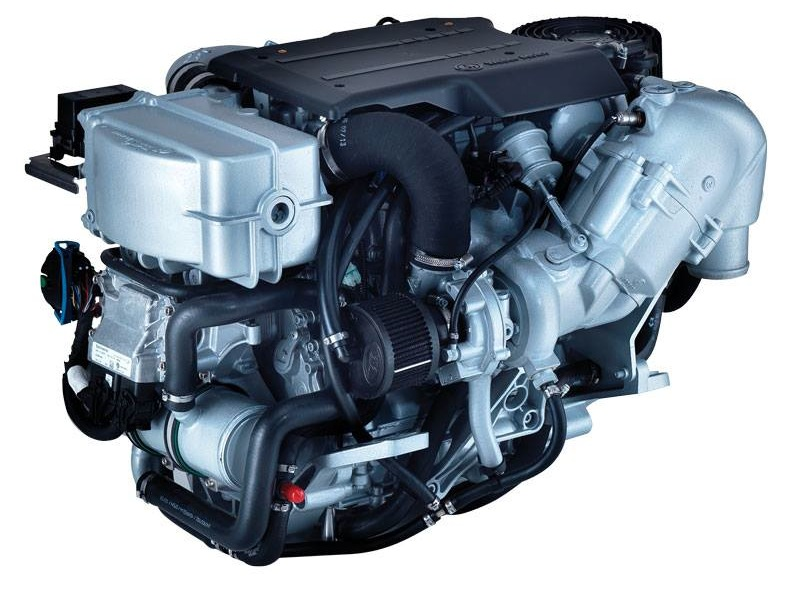
\includegraphics[width=\textwidth]{weber_MPE_850.jpg}
            \caption{Weber MPE 850 maritime motor. Adapted from \autocite{shawWeberMPE8502014}}
            \label{fig:weber_motor}
        \end{subfigure}
        \hfill
        \begin{subfigure}{0.48\textwidth}
            \centering
            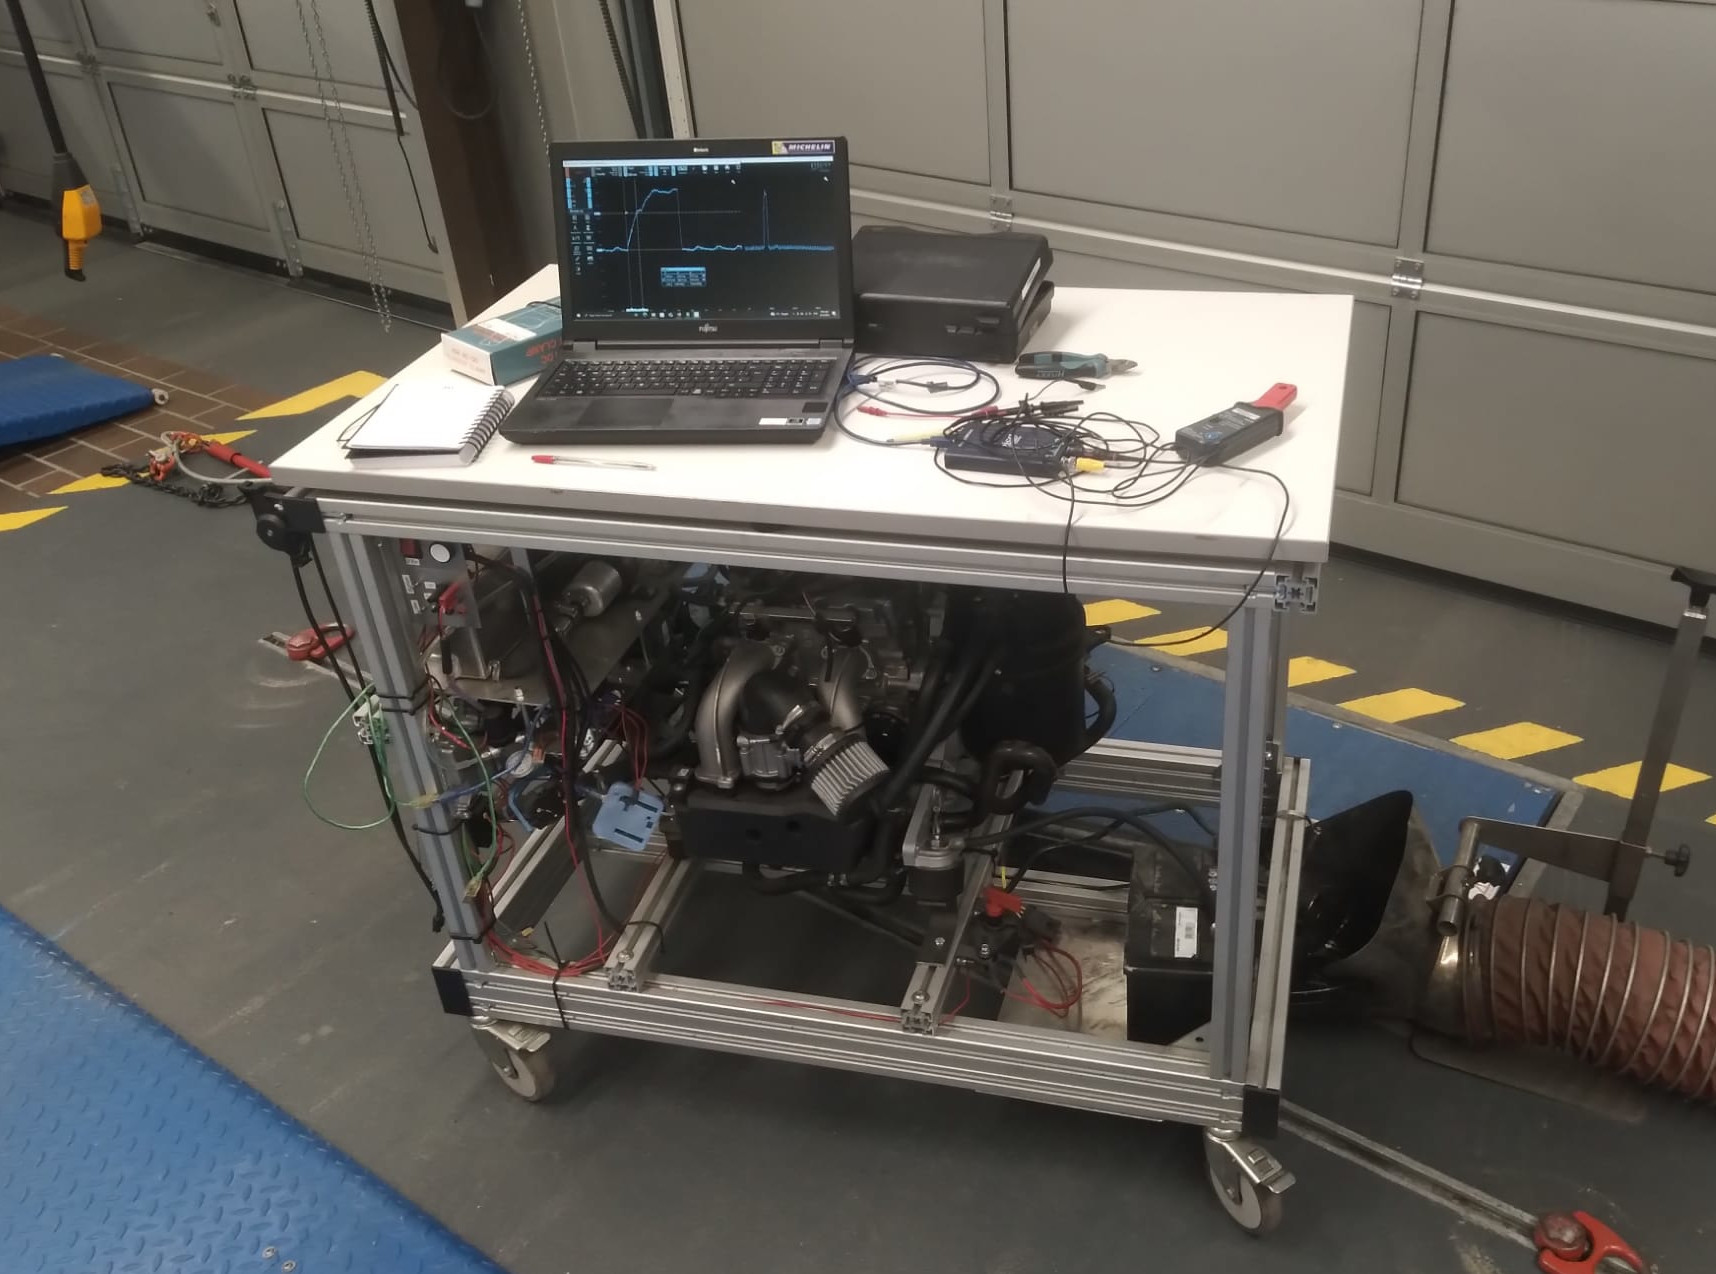
\includegraphics[width=\textwidth]{measurement_setup_preparation.jpeg}
            \caption{Motor ready for testing}
            \label{fig:measurement_setup}
        \end{subfigure}
        \caption{Test motor and measurement setup for injector characterization}
        \label{fig:motor_and_setup}
    \end{figure}

    %% todo: add more information about the motor

    When inspecting the motor during the first tests, several issues were found. Some fuel lines had to be replaced due to small leaks, and the fuel pressure was not high enough, resulting in very lean combustion (the motor has no lambda closed loop control). The fuel pressure was adjusted according to the motor installation manual to 4 bar \autocite{textronmotorsgmbhINSTALLATIONMANUAL4Stroke2013}. The tachometer of the motor was also reading incorrectly, consistently showing exactly half of the real RPM. This could be due to the fact that the Weber motor does not use \gls{wasted_spark} on the ignition system. The motor RPM for the next measurements was deduced from the injection signal, which was measured with an oscilloscope. 
    
    The Innovate LM2 AFR meter that had been used in previous tests also malfunctioned, so it could not be used for the measurements. A MAHA MET 6.3 emission tester was used instead.

    Having the motor at hand, the next step was to characterize the injectors and the ECU injector driver. This was done by measuring current and voltage at the injectors' terminals in different operating conditions. From these measurements, the DC resistance and inductance of the injectors were estimated, which are crucial parameters for the module design. 

    It is important to note that the injector parameters are also needed to emulate the injectors for the \gls{ecu}s to accept the modification. Modern \gls{ecu}s have diverse diagnostic mechanisms to ensure that the multiple systems in the motor are functioning properly, including the injectors. Upon testing, it was found that for the specific \gls{ecu}s used in the Weber motor, the control unit only needs to have a resistance of similar value to that of the injector, and no inductance is required. This means that the module can be designed to emulate the injectors as resistors, which simplifies the design. The resistors will have to dissipate a considerable amount of power, depending on the \gls{duty_cycle} of the injectors (analogous to the \gls{injection_pulse_width}), so they will have to be chosen accordingly.

    \section{Injector Characterization}

    The current was measured with a TA018 Current Clamp (60A AC/DC) connected to a PicoScope 2204A PC Oscilloscope, and the resistance was measured using a Fluke 1279 TRUE RMS Multimeter. The measurements were conducted with the motor running at different RPMs and various injection pulse widths. All measurements were performed with the battery voltage stable at approximately 12 V to ensure consistent results.

    %% figure with the comparison of the ideal curve and the measured curve (insert)

    \begin{figure}
        \centering
        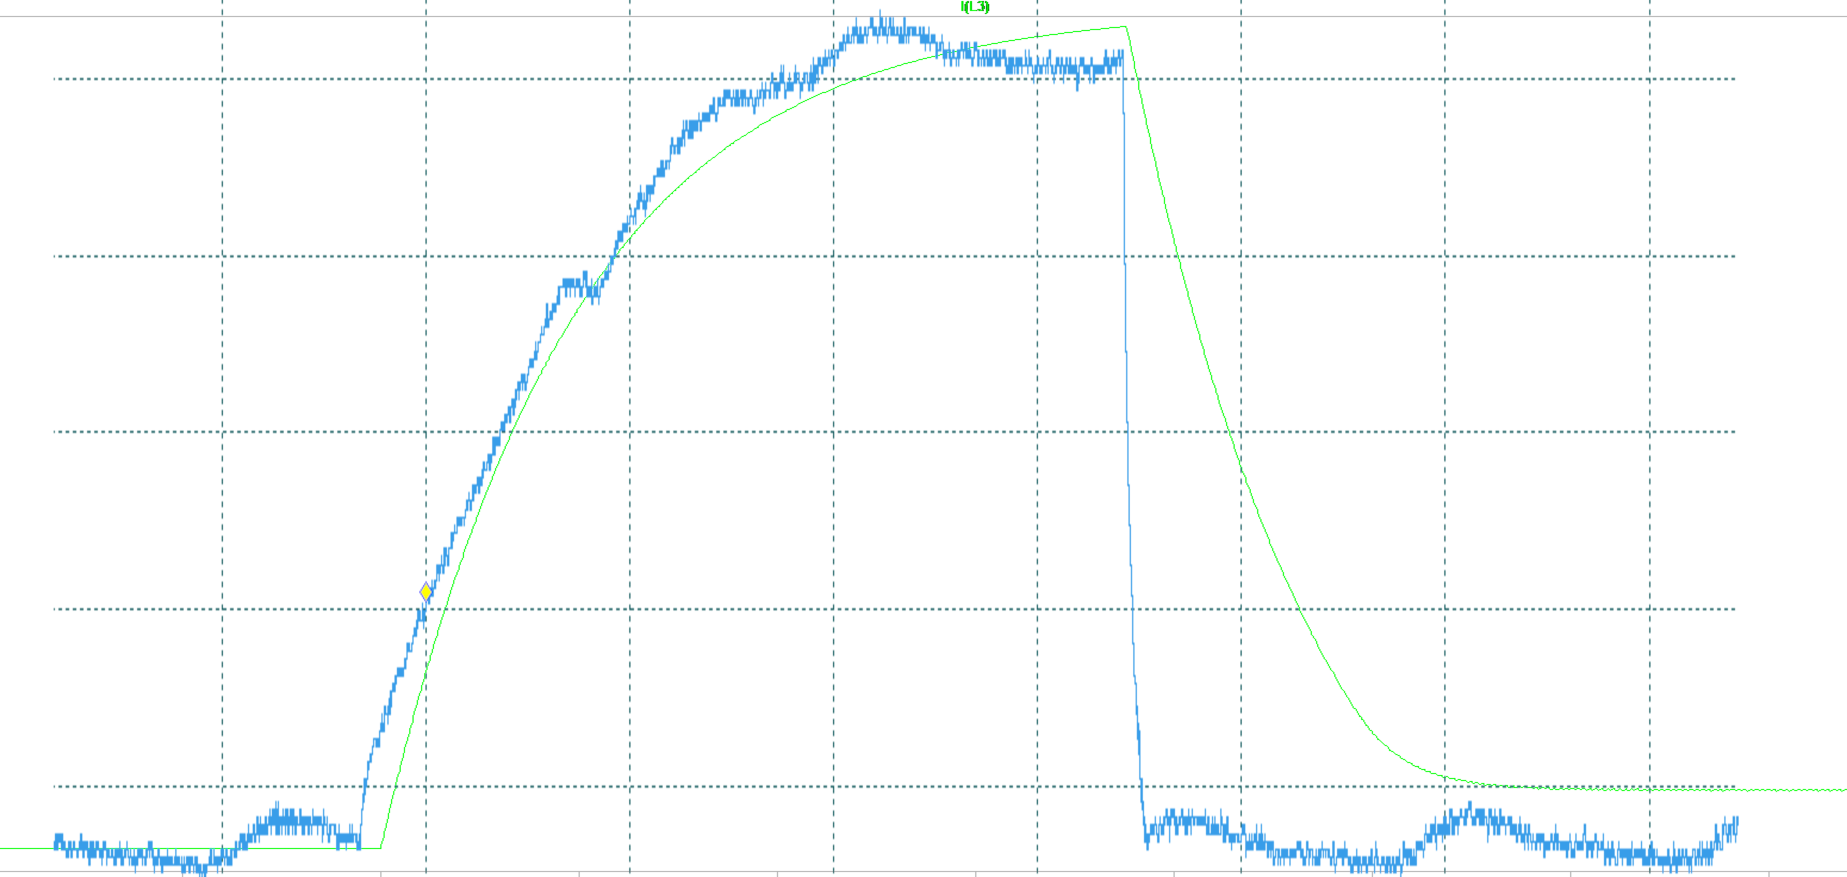
\includegraphics[width=0.8\textwidth]{graphs.png}
        \caption{Injector Characterization: measured current (blue) vs simulated current (green)}
        \label{fig:injector_characterization}
    \end{figure}

    In Figure \ref{fig:injector_characterization}, some noise due to the motor's other peripherals is visible, but the general trend is clear. The injector current (in blue) rises for approximately $1$ ms up to a visible peak, and then continues to rise until reaching the saturation value. This intermediate peak denotes the opening time of the injector \autocite{wieclawskiElectricCurrentWaveform2020}. It can also be confirmed that the injector is a high-impedance injector (around $12$ $\Omega$), as the current does not rise above $1$ A with a driving voltage of 12 V.

    The inductance of the injector can be calculated from the first \gls{time_constant} of the current rise, which is the time it takes for the current to rise from 0 to 63.2\% of its final value. For an RL circuit with a step voltage input:
    
    \begin{equation}
        \tau = \frac{L}{R} 
    \end{equation}
    
    From the measured values, an inductance of approximately $12$ mH was estimated. This is based on multiple measurements of the first time constant, which ranged from 817 µs to 1216 µs, with an average DC resistance of 12.3 $\Omega$. These values are in line with the literature for similar injectors \autocite{wieclawskiElectricCurrentWaveform2020} \autocite{texasinstrumentsLM1949InjectorDrive1995} \autocite{linearProductsDatasheet}.

    \begin{table}[H]
        \centering
        \caption{Injector Characterization Measurements}
        \label{tab:injector_measurements}
        \begin{tabular}{|c|c|c|c|c|c|}
            \hline
            \textbf{R ($\Omega$)} & \textbf{I$_{max}$ (mA)} & \textbf{$\tau$ (µs)} & \textbf{L (mH)} & \textbf{T$_{open}$ (ms)} & \textbf{T$_{high}$ (ms)} \\
            \hline
            12.3 & 891.4 & 817.2 & 10.05 & 1.197 & 3.779 \\
            12.3 & 895.5 & 1216.0 & 14.96 & 1.180 & 3.758 \\
            12.3 & 896.0 & 1059.0 & 13.03 & 1.174 & 3.766 \\
            12.3 & 892.0 & 930.6 & 11.45 & 1.170 & 3.747 \\
            12.3 & 883.0 & 981.6 & 12.07 & 1.176 & 3.788 \\
            12.3 & 817.7 & 993.0 & 12.21 & 1.263 & 3.543 \\
            12.3 & 783.2 & 970.1 & 11.93 & 1.277 & 3.034 \\
            \hline
            \textbf{Average} & \textbf{865.5} & \textbf{995.4} & \textbf{12.24} & \textbf{1.205} & \textbf{3.631} \\
            \hline
        \end{tabular}
    \end{table}

    % include figure for the inductive kickback
    \begin{figure}[H]
        \centering
        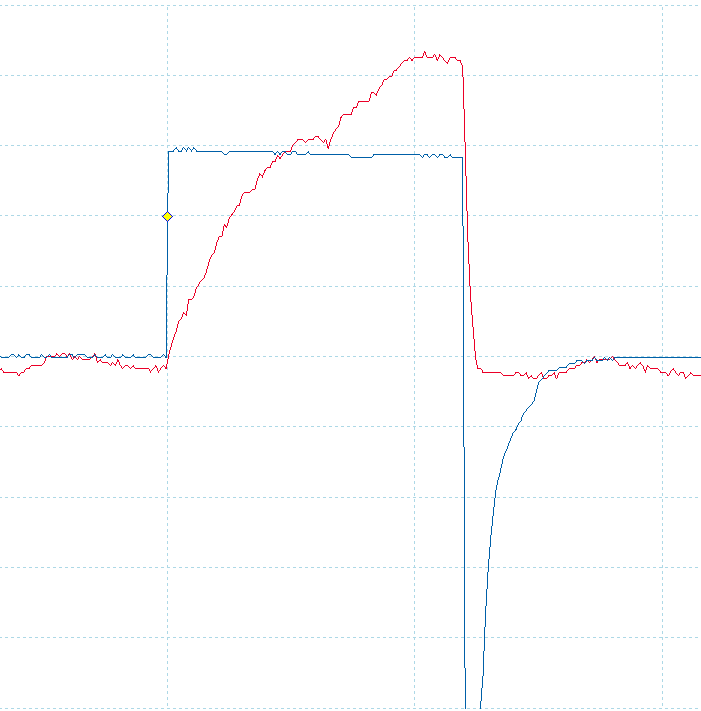
\includegraphics[width=0.5\textwidth]{inductive_kickback.png}
        \caption{Inductive Kickback from the Injector}
        \label{fig:inductive_kickback}
    \end{figure}

    The measured opening time of the injectors was consistently around 1.2 ms, which corresponds to the visible peak in the current profile \autocite{wieclawskiElectricCurrentWaveform2020}. This observation further supports the hypothesis that the injectors in the Weber motor are high-impedance injectors, as low-impedance injectors typically have a much shorter opening time.

    From Figure \ref{fig:inductive_kickback}, we can also make conjectures about the driver in the \gls{ecu}. The current drops drastically after the injector is shut off, which indicates that the driver employs an active clamping topology. This rapid demagnetization time ($T_{DEMAG}$) is an important parameter for injector control.

    The demagnetization time in an inductive circuit can be calculated by solving for when the total current decays to zero \autocite{texasinstrumentsHowDriveResistive2021,kerscherFasterSwitchingLarge2022}. 

    \begin{equation}
        T_{DEMAG} = \frac{L}{R} * \ln(1 + \frac{R * I_0}{V_{CLAMP} - V_{BAT}})
    \end{equation}

    Where:
    \begin{itemize}
        \item $L$ is the inductance of the injector
        \item $R$ is the resistance of the injector
        \item $I_0$ is the initial current at turn-off
        \item $V_{CLAMP}$ is the clamping voltage
        \item $V_{BAT}$ is the battery voltage
    \end{itemize}

    The rapid decay observed in the measurements indicates a relatively high clamping voltage compared to the battery voltage, which effectively reduces demagnetization time. The downside of such a high clamping voltage is that the injector driver output stage needs to handle higher \gls{avalanche} power (energy released by the collapse of the magnetic field in the inductor).



